\section{Experimental Results}



\subsection{Experimental Setup}
\begin{frame}[red] %hmm.. thought i could change colour here :S
\frametitle{Experimental Setup} 
\begin{itemize}
\item Query logs divided equally into 2 sets: 
  \begin{itemize}
    \item historical
    \item query workload
  \end{itemize}
\item Comparison with:
  \begin{itemize}
    \item Least Recently Used (LRU)
    \item Higest Query Frequency (HQF)
  \end{itemize}  
\end{itemize}

\begin{tabular}{c|cc}\hline
Dataset & Trajectories & Road network \\ \hline \hline
Aalborg & Infati GPS data &  From {\em downloads.cloudmade.com} \\
        & 4,401 trajectories  & 129k nodes, 137k edges \\\hline
Beijing & Geo-Life GPS data & From {\em downloads.cloudmade.com} \\
        & 12,928 trajectories & 76k nodes,  85k edges \\\hline
\end{tabular}

%Say why we use LRU/HQF "they are typical methods used in the caching area"

\end{frame}


\subsection{Hit ratio}
\begin{frame}[plain]%hmm.. thought i could change colour here :S
\frametitle{Hit ratio | Proxy Scenario} 

\center \hspace{-3em}
  \begin{tabular}{cc}
     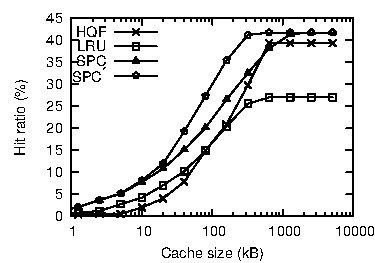
\includegraphics[width=0.5\columnwidth]{images/cachesize_hitratio_aal.pdf}
     &
     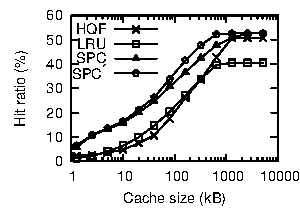
\includegraphics[width=0.5\columnwidth]{images/cachesize_hitratio_bei.pdf}
      \\
     Aalborg & \hspace{4em} Beijing
     \end{tabular}
\end{frame}


\subsection{Performance Savings}
\begin{frame}[plain]%hmm.. thought i could change colour here :S
\frametitle{Performance Savings | Server Scenario} 

  \begin{tabular}{ccc}
    \begin{sideways}Dijkstra \end{sideways} &
     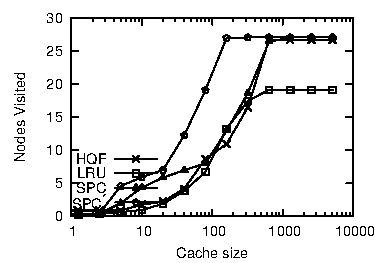
\includegraphics[width=0.45\columnwidth]{images/cachesize_diffnodes_aal_server.pdf}
     &
     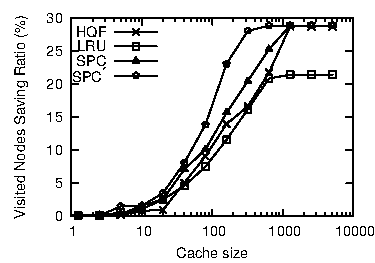
\includegraphics[width=0.45\columnwidth]{images/cachesize_diffnodes_bei_server.pdf} \\
     & Visited nodes savings, Aalborg & Visited nodes savings, Beijing \\

     \begin{sideways}A$^*$ \end{sideways} &
     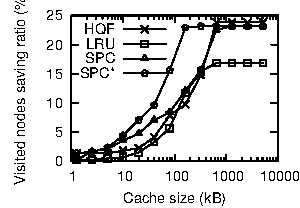
\includegraphics[width=0.45\columnwidth]{images/cachesize_diffnodes_aal_server_astar.pdf}
     &
     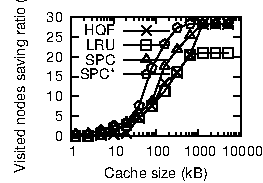
\includegraphics[width=0.45\columnwidth]{images/cachesize_diffnodes_bei_server_astar.pdf} \\
     & Visited nodes savings, Aalborg & Visited nodes savings, Beijing \\
  \end{tabular}
\end{frame}


\begin{frame}[plain]%hmm.. thought i could change colour here :S
\frametitle{Performance Savings | Server Scenario} 
  \begin{tabular}{ccc}
    \begin{sideways}Dijkstra \end{sideways} &
     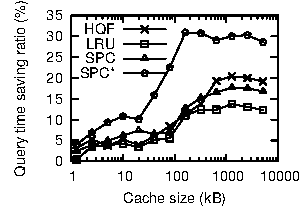
\includegraphics[width=0.45\columnwidth]{images/cachesize_diffruntime_aal_server.pdf}
     &
     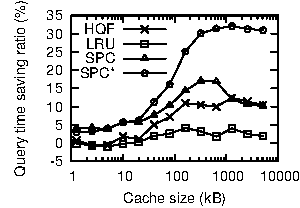
\includegraphics[width=0.45\columnwidth]{images/cachesize_diffruntime_bei_server.pdf} \\
     & Query time savings, Aalborg & Query time savings, Beijing \\

     \begin{sideways}A$^*$ \end{sideways} &
     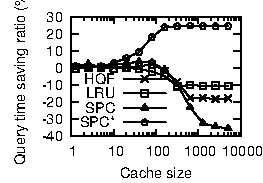
\includegraphics[width=0.45\columnwidth]{images/cachesize_diffruntime_aal_server_astar.pdf}
     &
     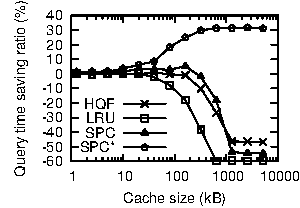
\includegraphics[width=0.45\columnwidth]{images/cachesize_diffruntime_bei_server_astar.pdf}
      \\
      & Query time savings, Aalborg & Query time savings, Beijing  \\
  \end{tabular}
\end{frame}
